% !TEX root = main.tex
\subsection{Beobachtung der Milchstraße}
Ziel dieses Auswertungsabschnitts ist es, die Rotationsgeschwindigkeit in der Milchstraße zu ermitteln und die Milchstraße zu kartografieren.\newline
Hierfür werden Radiowellen bei $\SI{1410}{\mega \hertz}$ untersucht. Diese Frequenz ist das Äquivalent zu der charakteristischen ,,$\lambda = \SI{21}{\centi \metre}$``-Linie des H1-Übergangs von Wasserstoff. Aufgrund der großen Menge an Wasserstoff in unserer Galaxie ist dieser eigentlich ,,verbotene`` Übergang mit dem Radioteleskop detektierbar.\newline
\subsubsection{Belichtungszeit}
Um die Milchstraße kartografieren zu können, müssen zunächst die richtigen Einstellungen an dem Radioteleskop getroffen werden. Mithilfe des \textit{Switched}-Modus, welcher das Rauschen minimiert und bei einer Bandbreite von \SI{2}{MHz} und 256 Kanälen und somit einer Frequenzauflösung von $\SI{7.8}{\kilo \hertz}$ pro Kanal \cite{Usermanual} wird dafür zunächst die Belichtungszeit variiert. Abbildung \ref{fig:Belichtungszeit} zeigt die gemessenen Spektren für sechs verschiedene Belichtungszeiten. Dabei ist deutlich erkennbar, dass bei einer Belichtungszeit von lediglich $\SI{1}{s}$ ein sehr großes Rauschen auftritt und Maxima im Spektrum nicht deutlich genug ausgemacht werden können. Jedoch glättet sich das Rauschen schon bei einer Belichtungszeit von $\SI{10}{\second}$ deutlich. Ab einer Belichtungszeit von $\SI{30}{\second}$ ist schon fast kein signifikanter Unterschied zu längeren Belichtungszeiten mehr erkennbar. Auf Einzeichnung der Unsicherheiten in den Abbildungen wurde in diesem Abschnitt verzichtet, da dies die Abbildung unleserlich machen würde. Jedoch werden die auftretenden Unsicherheiten stets diskutiert und werden somit dennoch berücksichtigt.
\begin{figure}[H]
    \centering
    \input{plots/Belichtungszeit.tex}   
    \caption[Gemessene Spektren bei verschiedenen Belichtungszeiten]{Mithilfe dieser Abbildung lässt sich erkennen, wie sich die gemessenen Spektren mit der Belichtungszeit verändern. Bei einer Belichtungszeit von $\SI{1}{\second}$ ist ein sehr ausgeprägtes Rauschen des Signals zu verzeichnen. Maxima sind bei dieser Belichtungszeit kaum ausmachbar. Das Rauschen ist allerdings schon bei einer Belichtungszeit von $\SI{10}{\second}$ deutlich reduzierter ausgeprägt. Maxima lassen sich bei dieser Belichtungszeit deutlich genauer ausmachen.}
    \label{fig:Belichtungszeit}
\end{figure}
Abbildung \ref{fig:BelichtungszeitExtremal} zeigt dafür nochmals die extremalen Belichtungszeiten für eine genauere Analyse der Spektren. Da sich das Spektrum ab einer Belichtungszeit von $\SI{30}{\second}$ nicht mehr merklich verändert, sind die Messungen stets mit einer Belichtungszeit von $\SI{60}{\second}$ aufgenommen. Somit ist es nochmal ein wenig genauer wie eine Messung bei $\SI{30}{\second}$, sprengt aber nicht den zeitlichen Rahmen des begrenzten Versuchszeitraums, was eine Messung bei jeweils $\SI{300}{\second}$ getan hätte.
\begin{figure}[H]
    \centering
    \input{plots/BelichtungszeitExtrema.tex}   
    \caption[Eindeutige Unterschiede der Spektren bei verschiedenen Belichtungszeiten]{Diese Abbildung soll noch einmal die eindeutigen Unterschiede der Spektren bei verschiedenen Belichtungszeiten verdeutlichen. Da sich das Spektrum bei einer Belichtungszeit von \SI{30}{\second} und \SI{300}{\second} nur noch minimal unterscheidet, wurde eine Belichtungszeit für die Spektren von $\SI{60}{\second}$ gewählt. Bei dieser Zeit waren alle Maxima deutlich ausmachbar und der zeitlich begrenzte Versuchszeitraum wurde nicht gesprengt.}
    \label{fig:BelichtungszeitExtremal}
\end{figure}
\subsubsection{Verarbeitung der Daten}
Mithilfe eines \textsc{MatLab}-Skripts wird das Untergrundrauschen der einzelnen Spektren geglättet und die auftretenden Peaks mittels einer \textsc{Gauß}-funktion gefittet. 
Somit lassen sich die Maxima sehr präzise bestimmen. 
Abbildung \ref{fig:TestBaseline} zeigt dieses Vorgehen exemplarisch. 
Dabei liegen die zwei Maxima bei \SI{7.3}{\frac{km}{s}} und \SI{-64.8}{\frac{km}{s}} relativ zu LSR, gemessen bei $l = \SI{30}{\degree}, \, b = \SI{0}{\degree}$. 
Um eine aussagekräftige Karte der Milchstraße zu erstellen, sind Messungen vom ersten Quadranten bis in den dritten Quadranten hinein vorgenommen worden.
\begin{figure}[H]
    \centering
    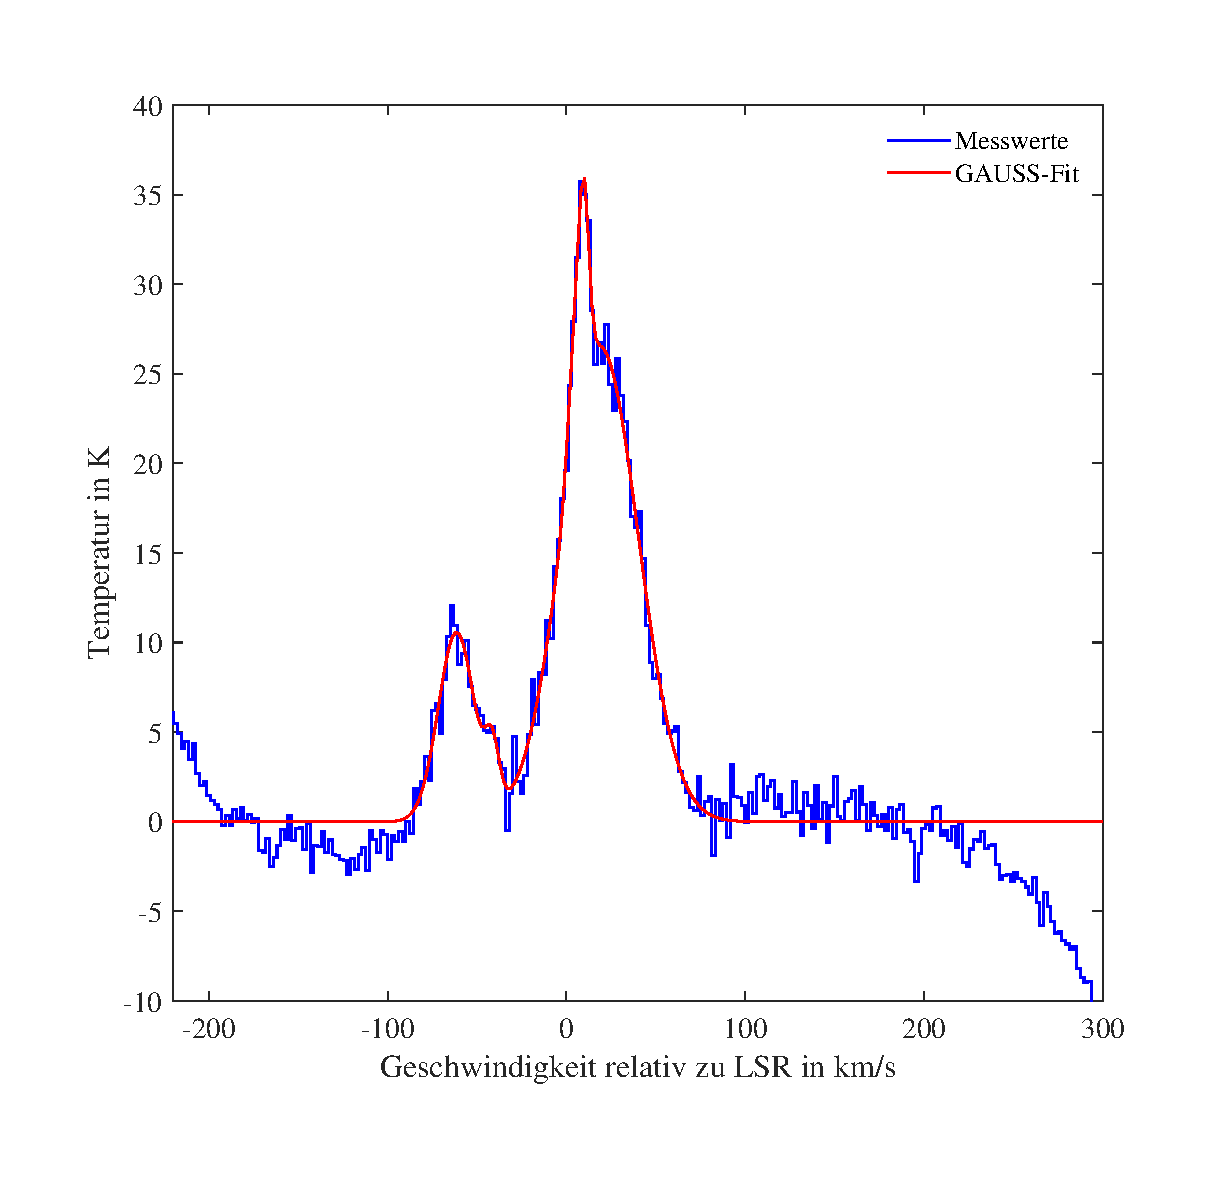
\includegraphics[width= 0.9\textwidth]{plots/TestBaseline.eps}
    \caption[Gemessenes Beispielspektrum zur Darstellung der Verarbeitung der Daten]{Gemessenes Beispielspektrum zur Darstellung der Verarbeitung der Daten. Da bei den Messungen stets ein Untergrundrauschen mitgemessen wurde, musste dieses mithilfe eines Computerprogramms herausgefiltert werden. Mittels eines \textsc{MatLab}-Skripts wurden die Spektren jeweils noch mit \textsc{Gauß}funktionen gefittet. So lassen sich die Maxima deutlich erkennen und auslesen. In diesem Fall handelt es sich um eine Messung bei $l = \SI{30}{\degree}, \, b = \SI{0}{\degree}$ und die beiden Maxima liegen bei \SI{7.3}{\frac{km}{s}} und \SI{-64.8}{\frac{km}{s}} relativ zu LSR.}
    \label{fig:TestBaseline}
\end{figure}
\subsubsection{Rotationsgeschwindigkeit}
Bevor die Milchstraße kartografiert wurde, sollte zunächst die Rotationsgeschwindigkeit einzelner Punkte in der Galaxie untersucht werden. Hierfür wurden aus den maximal verschobenen Maxima $V_{r,max}$ der Geschwindigkeiten aus dem ersten Quadranten hin zu positiven Werten jeweils die Geschwindigkeit relativ zu LSR ausgelesen. Da es sich bei diesen Maxima um Tangentenpunkte handelt, kann der Radius $R$ zum Zentrum der Milchstraße wie folgt ermittelt werden \cite{H1}:
\begin{align}
    R = R_0 \cdot \sin(l) \ .
    \label{eq:TangenteR}
\end{align}
Hierbei ist $R_0 = \SI{8.5}{\kilo \parsec}$ der Abstand der Sonne zum Zentrum der Milchstraße. Die Werte für $R$ lassen sich aus der Tabelle \ref{tab: erster Quadrant} entnehmen. Mithilfe von $R$ lässt sich nun auch die Geschwindigkeit mit folgender Gleichung \cite{H1}
\begin{align}
    V = V_{r,max} + V_0 \cdot \sin(l)
    \label{eq:V(R)}
\end{align}
ermitteln. Die Werte dafür können ebenfalls der Tabelle \ref{tab: erster Quadrant} entnommen werden. Abbildung \ref{fig:VvonR} zeigt die Rotationsgeschwindigkeiten, aufgetragen über dem korrespondierenden Bahnradius. Dabei ist ersichtlich, dass diese nahezu linear angeordnet sind. Mithilfe eines linearen Fits lässt sich der Mittelwert von $\SI{210.9 \pm 3.1}{\frac{km}{s}}$ ausmachen, welcher beinahe in Übereinstimmung mit dem Literaturwert von $\SI{220}{\frac{km}{s}}$ \cite{LSR} ist. Ein linearer Verlauf ist für Rotationsgeschwindigkeiten von Planeten ungewöhnlich, da entweder ein linearer Zusammenhang ($V \sim R$) wie bei einem starren Körper oder ein $V \sim\frac{1}{\sqrt{R}}$ wie bei einer Zentralmasse zu erwarten ist. Ohne diesen Zusammenhang wäre die Milchstraße nicht stabil. Die konstante Geschwindigkeit lässt sich nur auf eine unbekannte Energie und Materie (schwarze  Energie/Materie) zurückführen, welche die Massen zusammenhält.
\begin{figure}[H]
    \centering
    \input{plots/VvonR.tex}
    \caption[Rotationskurve der Milchstraße]{Dargestellt ist eine Rotationskurve der Milchstraße. Die eingetragenen Datenpunkte wurden jeweils aus dem Peak der maximal verschobenen Geschwindigkeitskomponente der gemessenen Geschwindigkeitsspekra aus dem ersten Quadranten gewonnen. Es ist deutlich zu erkennen, dass die Geschwindigkeit $V(R)$ nahezu unabhängig von dem Bahnradius ist. Mit einem linearen Fit wurde dies in der Abbildung nochmals verdeutlicht. Der Ordinatenabschnitt kennzeichnet dabei den Mittelwert der gemessenen Geschwindigkeiten. Dieser beträgt $\SI{210.9 \pm 3.1}{\frac{km}{s}}$ und kommt einem Literaturwert von $\SI{220}{\frac{km}{s}}$ \cite{LSR} sehr nahe. Einen exakten Literaturwert für die Geschwindigkeit zu finden, ist nicht möglich, da dieser bei verschiedenen Quellen unterschiedlich angegeben wird. Jedoch wird immer ein Wert um $\SI{220}{\frac{km}{s}}$ angegeben.}
    \label{fig:VvonR}
\end{figure}
\subsubsection{Kartografie der Milchstraße}
Da die Rotationsgeschwindigkeit nahezu konstant ist, wird im Folgenden eine Geschwindigkeit von $V(R) = V_0 = \si{220}{\frac{km}{s}}$ angenommen. Mithilfe dieser Annahme kann nun für jedes Maxima aus den Spektren der jeweilge Radius $R$ wie folgt ermittelt werden \cite{H1}:
\begin{align}
    R =\frac{R_0 \cdot V_0 \cdot \sin(l)}{V_0 \cdot \sin(l) + V_r} \ .
    \label{eq:BerechnungR}
\end{align}
Hierbei ist $V_r$ das jeweilge Maximum im Spektrum relativ zu LSR.\newline
Mit $R$ kann nun mithilfe des Cosinussatzes ein Ausdruck für $r$ (Abstand Sonne-Wasserstoffwolke) ermittelt werden \cite{H1}:
\begin{align}
    r_{\pm} = \pm \sqrt{R^2 - R_0^2 \cdot \sin(l)^2} + R_o \cdot \cos(l) \ .
    \label{eq:Berechnungr}
\end{align}
Negative Werte für $r$ können vernachlässigt werden, da dies bedeutet, dass sie sich hinter der Sonne befinden würden \cite{H1}. Da es im ersten Quadranten ($ \si{0}{\degree} \le l \le \si{90}{\degree}$) allerdings mehrere positive Lösungen für $r$ gibt, muss eine genauere Untersuchung der Beobachtungsrichtung gemacht werden. 
Hierfür wird die galaktische Breite $b$ variiert. Somit sollten Wasserstoffwolken, welche weiter entfernt liegen, nicht mehr als Peak im Spektrum sichtbar sein, da sie dann außerhalb des Beobachtungsfensters liegen. Die Abbildung \ref{fig:bungleichnull} zeigt exemplarisch eine Aufnahme bei $b \neq 0$. Es ist erkennbar, dass trotz der Wahl von $b = \pm 2$ alle Maxima ersichtlich sind. Somit kann keine weitere Aussage über $r$ getroffen werden. Da am Versuchstag allerdings nur Untersuchungen bis $b = \pm 2$ gemacht worden sind, wurde auf alle Werte, für die zwei positive Ergebnisse für $r$ existieren, verzichtet. Für alle anderen Werte lassen sich die Ergebnisse für $r_{\pm}$ aus den Tabellen \ref{tab: erster Quadrant}, \ref{tab: zweiter Quadrant1} und \ref{tab: zweiter Quadrant2} entnehmen.
\begin{figure}[H]
    \centering
    \input{plots/bungleichnull.tex}   
    \caption[Spektren für verschiedene galaktische Breiten $b$]{Diese Abbildung zeigt Spektren für verschiedene galaktische Breiten $b$. Erkennbar ist, dass in allen Spektren stets bei allen gewählten galaktischen Breiten $b$ die Maxima bei \SI{2.4}{\frac{km}{s}}, \SI{-30.6}{\frac{km}{s}} und \SI{-69.7}{\frac{km}{s}} erkennbar sind. Die Werte für $b$ sind offenbar zu klein gewählt worden. Bei größeren galaktischen Breiten sollte mindestens ein Peak weniger auftreten. Auf Fits mittels \textsc{Gauß}-Funktionen wurde bei dieser Abbildung zu Gunsten der besseren Lesbarkeit verzichtet.}
    \label{fig:bungleichnull}
\end{figure}
Die ermittelten Koordinaten $r$ lassen sich nun noch in kartesische Koordinaten transformieren. Dies geschieht mit nachfolgenden Gleichungen \cite{H1}:
\begin{align}
    x &= r \cdot \cos(l-90\degree) \\
    y &= r \cdot \sin(l-90\degree) 
    \label{eq:umrechnung}
\end{align}
Die so ermittelten Werte lassen sich wieder aus den Tabellen \ref{tab: erster Quadrant}, \ref{tab: zweiter Quadrant1} und \ref{tab: zweiter Quadrant2} entnehmen.\newline
Nun können alle ermittelten Werte in eine zweidimesionale Abbildung eingetragen werden, wie in Abbildung \ref{fig:Milchstrassesafe} zu sehen. In dieser Abbildung sind teilweise deutliche Strukturen der Milchstraße analog zur Literatur (siehe Abbildung \ref{fig:Milchstrasselit}) zu sehen.
Zu beachten ist, dass Abbildung \ref{fig:Milchstrasselit} galaktische Koordinaten verwendet und die ertellte Abbildung \ref{fig:Milchstrassesafe} das kartesische Koordinatensystem verwendet.
Da allerdings die Milchstraße stets eine galaktische Breite von $b= \si{0}{\degree}$ aufweist, können die beiden verschiedenen Koordinatensysteme problemlos in einer zweidimensionalen Abbildung miteinander verglichen werden.\newline
Da in diesem Bericht nur in einem Bereich von $\si{33}{\degree} \le l \le \si{203}{\degree}$ gemessen wurde, sind keine Datenpunkte im vierten Quadrant und nur wenige Datenpunkte im dritten Quadrant zu sehen.
Werden allerdings die Datenpunkte des ersten Quadranten genauer betrachtet, so ergibt ein Vergleich mit der Literatur, dass es sich vermutlich um den \textit{Cygnus-Arm} handelt. Bei den Datenpunkten um den Koordinatenursprung ist es deutlich schwieriger, eine eindeutige Aussage zu treffen, da hier die Galaxiearme sehr dicht beieinanderliegen. Jedoch sind Tendenzen der Galaxiearme \textit{Perseus} und \textit{Orion} zu erkennen. Bei den einzelnen Messpunkten bei $(x,y)=(-12.96, 30.54)$, $(x,y)=(48.82, 159.69)$ und $(x,y)=(-6.32, 14.89)$ handelt es sich vermutlich um Messpunkte, die ,,falsch`` sind. Dies ist darauf zurückzuführen, dass die Maxima in den Spektren nicht immer deutlich ersichtlich sind. Die blau markierte Fläche in Abbildung \ref{fig:Milchstrassesafe} charakterisiert die gesamte Fläche der Galaxie, welche einen Kreis mit einem Radius von etwa $\SI{25}{\kilo \parsec}$ einnimmt.
\begin{figure}[H]
    \centering
    \input{plots/Milchstrassesafe.tex}   
    \caption[Abbildung der Milchstraße]{In dieser Abbildung ist die Milchstraße mithilfe der Daten aus den Frequenzspektren kartografiert. Bei der Abbildung ist ein Seitenarm der Milchstraße im Bereich um $(x,y)=(10,-10)$ deutlich ersichtlich. Ein weiterer Galaxiearm ist im Bereich $(x,y)=(10,5)$ erkennbar, wobei dieser schon deutlich schwächer ausgeprägt ist. In dem Bereich um den Ursprung sind die Datenpunkte sehr dicht angehäuft. Somit ist in diesem Bereich leider keine eindeutige Aussage über etwaige Galaxiearme zu machen. Mithilfe des eingefärbten Kreises mit dem Radius von $\SI{25}{\kilo \parsec}$ ist die Größe der gesamten Galaxie ersichtlich.}
    \label{fig:Milchstrassesafe}
\end{figure}
\begin{figure}[H]
    \centering
    \includegraphics[width= 0.7\textwidth]{pngplots/milchstrasselit.png}   
    \caption[Literaturbeispiel zur Abbildung der Milchstraße]{Literaturbeispiel zur Abbildung der Milchstraße. Zu sehen sind die einzelnen Seitenarme (blau markiert) der Milchstraße, welche mit ihren Namen gekennzeichnet sind, und die Rotationsrichtung der gesamten Milchstraße. Für die Einordnung der Größenordnung ist noch ein Maßstab angegeben. \cite{H1}}
    \label{fig:Milchstrasselit}
\end{figure}